%\begin{figure}[p]
%    \centering
%    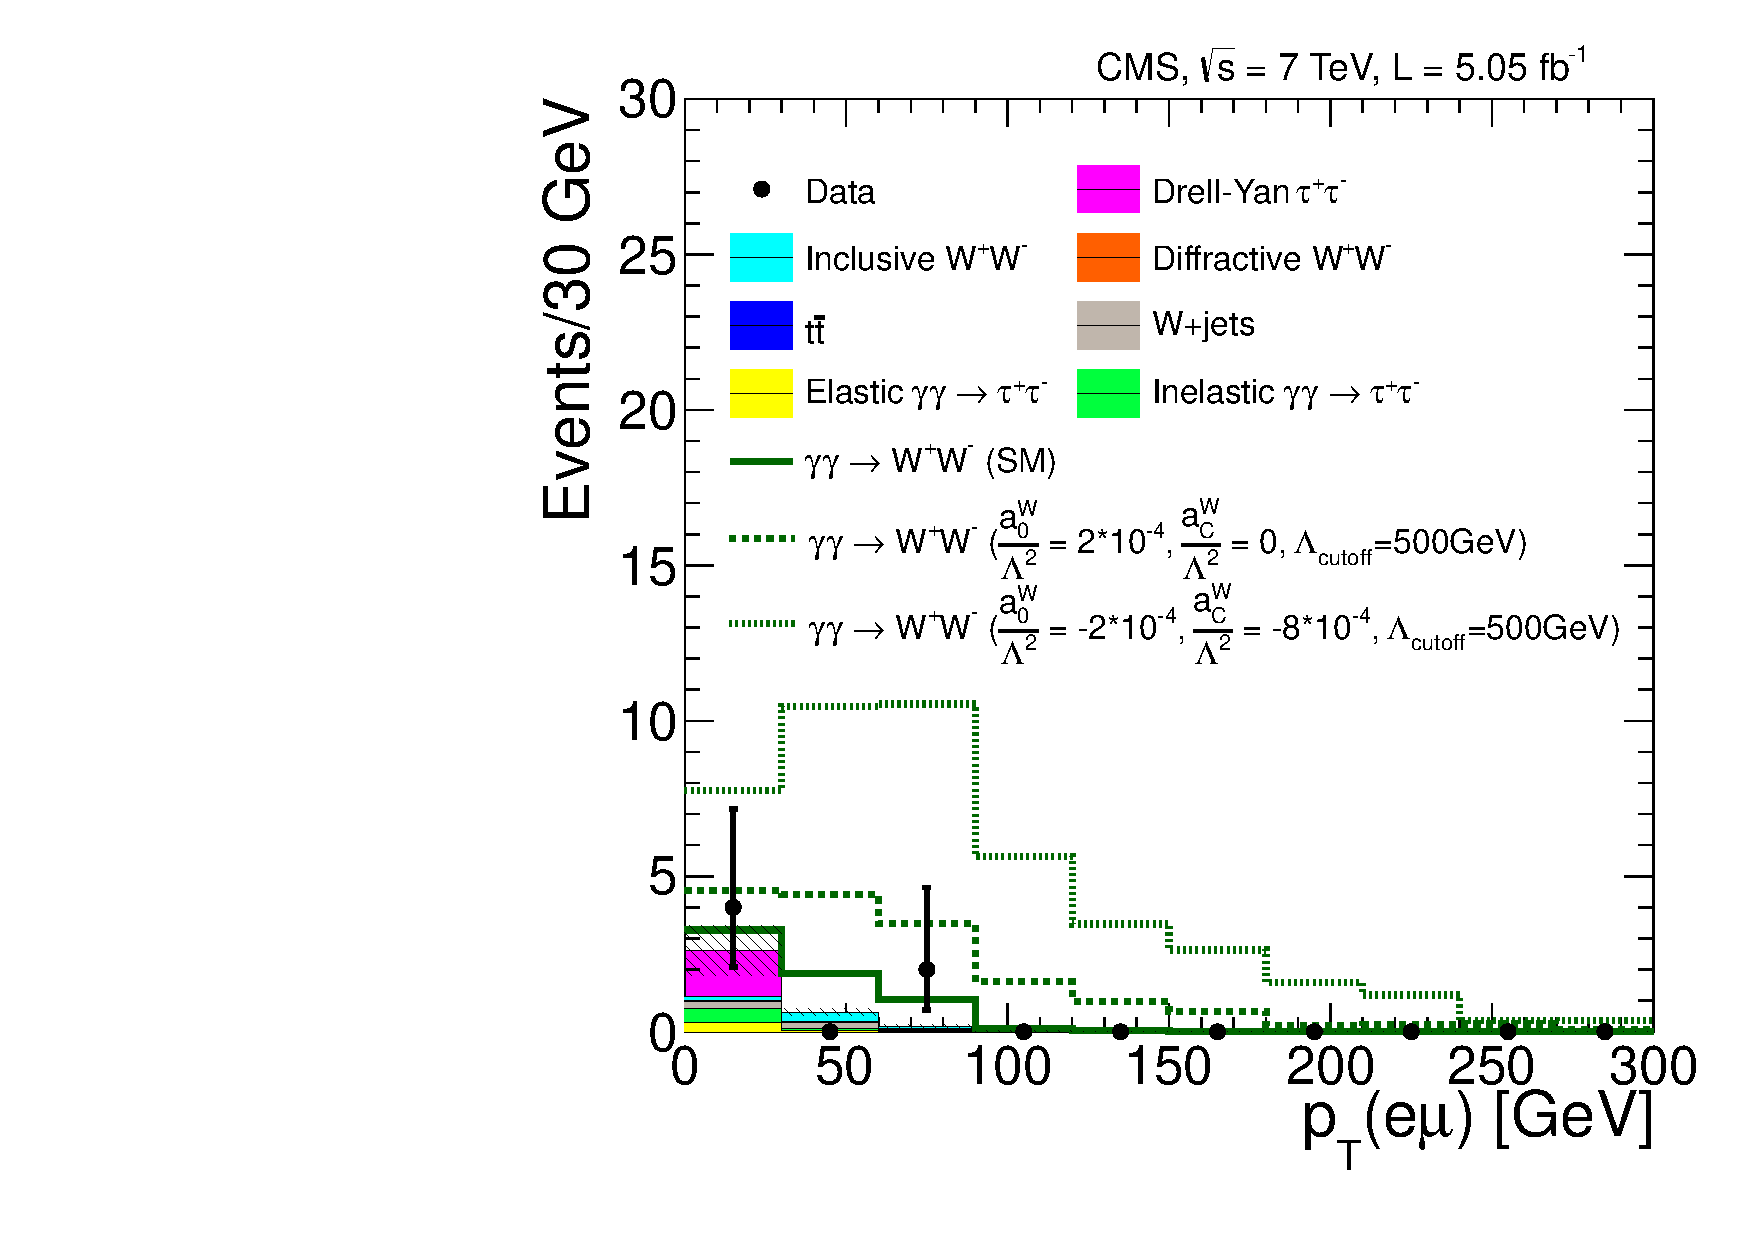
\includegraphics[height=0.3\textheight]{figures/ss-exclboson-ww-cms7tev}
%    \caption{}
%    \label{fig:ss-exclboson-ww-cms7tev}
%\end{figure}
%CMS WWexcl 7 \TeV~\cite{Chatrchyan:2013foa}

In addition to exclusive single boson production, CMS and ATLAS have evidence for exclusive diboson production, in two different channels.
In one of them, CMS has performed a search for exclusive diboson production via protons emitting (possibly quasi-) real photons which rescatter to produce $W^+W^-$ pairs:
$pp \to p^{(*)}W^+ W^- p^{(*)} \to p^{(*)}\mu^{\pm}e^{\mp}p^{(*)}$, where $p^*$ admits the possibility that the protons dissociate into an undetected system.
Such production is characterized by a $\mu^{\pm}e^{\mp}$ pair which has no underlying event activity typical of proton-proton hard scattering.
By selecting a $\mu^{\pm}e^{\mp}$ pair of sufficiently high individual (20 GeV) and joint (30 GeV) transverse momentum,
and requiring further that the two lepton tracks intersect with each other, but have no additional tracks nearby, an exclusive production signal is isolated from backgrounds such as
exclusive Drell-Yan and inclusive dilepton production from various hard scattering mechanisms, respectively.  Selection efficiency is validated by examining a control sample of
exclusive same-flavor Drell-Yan production ($p^{(*)}\mu^{\pm}\mu^{\mp}p^{(*)}$ or $p^{(*)}e^{\pm}e^{\mp}p^{(*)}$) and comparing it with simulated efficiency.
The relative contribution of dissociated proton scattering for signal is also deduced by comparing the observed exclusive Drell-Yan cross section with an exclusive
matrix element calculation (\texttt{LPAIR}); proton dissociation is estimated to enhance the signal by a factor of $4.10 \pm 0.43$ with respect to an exclusive calculation from \texttt{MadGraph}.

Figure~\ref{fig:ss-exclboson-ww-cms8tev} shows the distributions of dilepton $\pt$ and extra tracks in data compared with expectations from simulation.  13 events are observed with an expected
background of $3.9\pm0.6$ in the 8 TeV data.  In the 7 TeV and 8 TeV data combined, a 3.4 $\sigma$ excess is observed over background as evidence
for exclusive (plus dissociative) $W^+W^-$ production.  The signal corresponds to a cross section in the 8 TeV data of $11.9^{+5.6}_{-4.5}$ fb, in agreement with a SM prediction of $6.9\pm0.6$ fb.
Exclusive $W^+W^-$ production is sensitive to $WW\gamma\gamma$ quartic couplings. The CMS analysis derived limits on the dimension 6 couplings $a^W_0/\Lambda^2$ and $a^W_C/\Lambda^2$ and, in the context
of dimension 8 EFT, the anomalous couplings $f_{M(0,1,2,3)}/\Lambda^4$.  The 95\% CL upper limits are $1.1(4.4)\times 10^{-4} \rm{GeV}^{-2}􀀀$ for $a^W_0/\Lambda^2$ ($a^W_C/\Lambda^2$),
and range from $2-17 \times 10^{-4} \rm{GeV}^{-4}$ for dimension 8 couplings, for models with no form factor.  This process is the single best constraint on $WW\gamma\gamma$ QGCs.

\begin{figure}[htb]
\centering
%\includegraphics[width=.48\textwidth]{Figures/2016_01_29_UpdatedPlots/ee_pt.pdf}
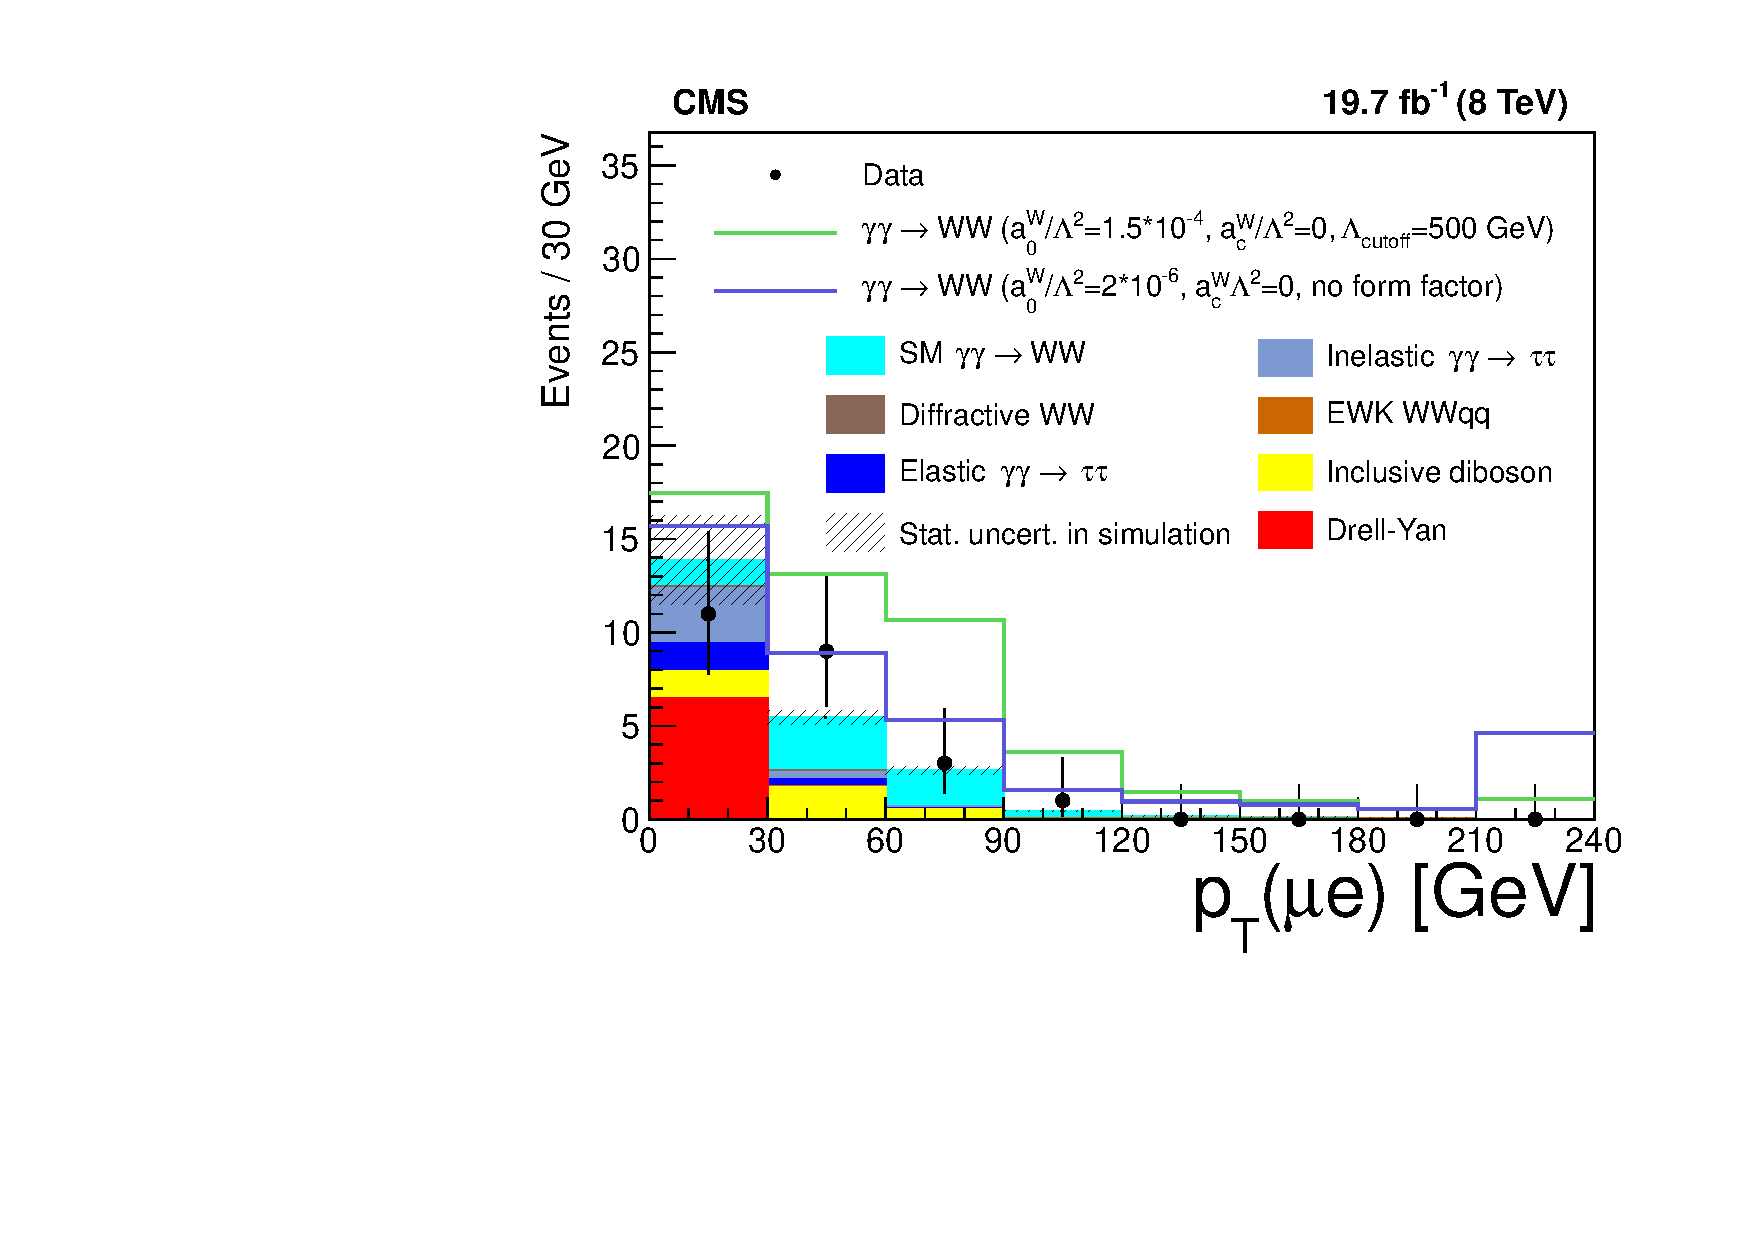
\includegraphics[width=.48\textwidth]{figures/ss-exclboson-ww-cms8tev-1.pdf}
%\includegraphics[width=.48\textwidth]{Figures/2016_01_29_UpdatedPlots/ee_tracks_
%pt30.pdf}
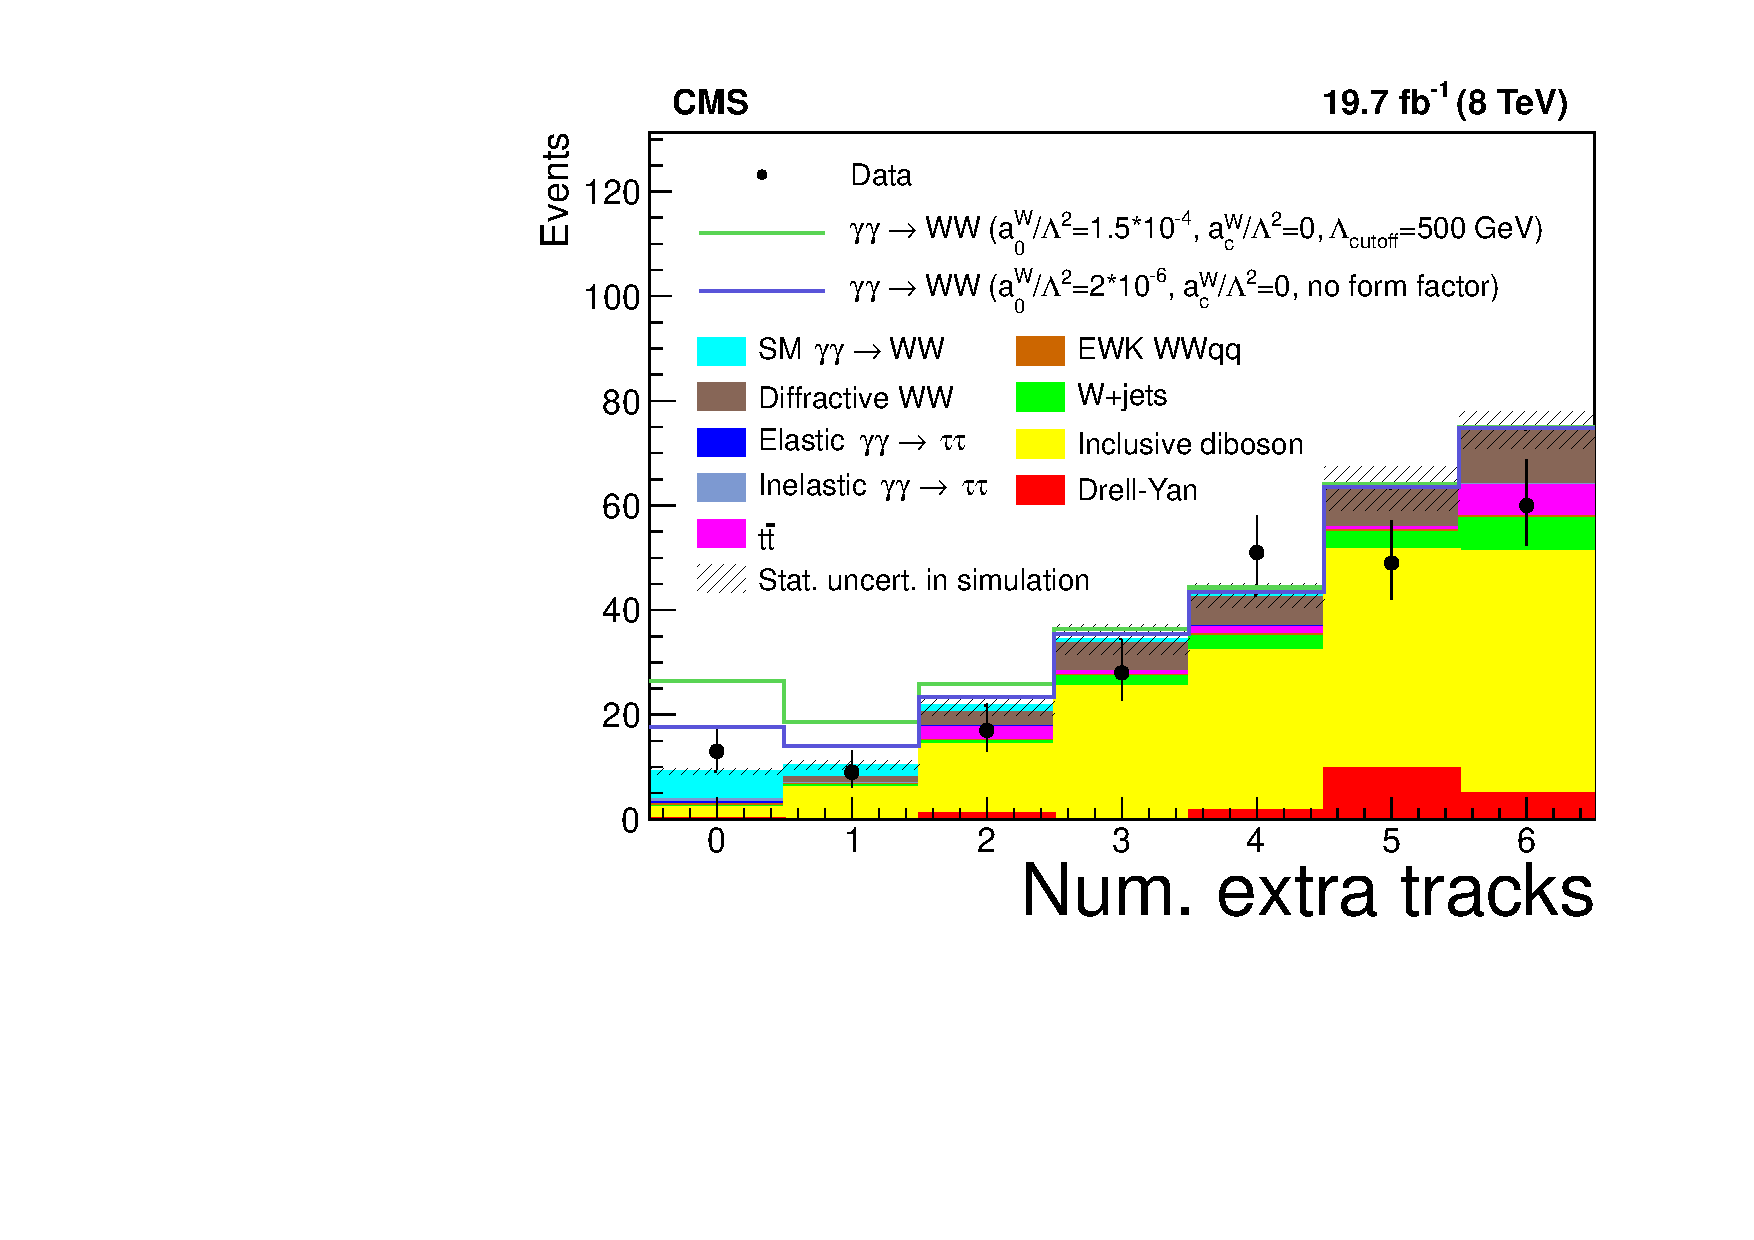
\includegraphics[width=.48\textwidth]{figures/ss-exclboson-ww-cms8tev-2.pdf}
\caption{Evidence for exclusive diboson production via $pp \to p^{(*)}W^+ W^- p^{(*)} \to p^{(*)}\mu^{\pm}e^{\mp}p^{(*)}$.
Distributions of muon-electron transverse momentum for events with zero
 associated tracks (left), and extra-tracks multiplicity for events with $\pt(\mu^{\pm}e^{\mp}) > 30$ GeV (right).
 The data are shown by the points with error bars; the histograms indicate the expected SM signal and backgrounds.
\label{fig:ss-exclboson-ww-cms8tev}}
\end{figure}




\begin{figure*}[htb] {
\centering
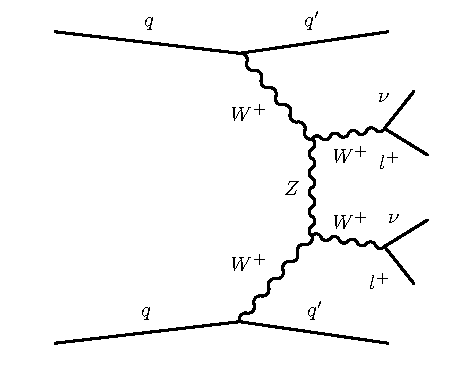
\includegraphics[width=0.315\textwidth]{figures/ss-exclboson-ww-diagram1.pdf}
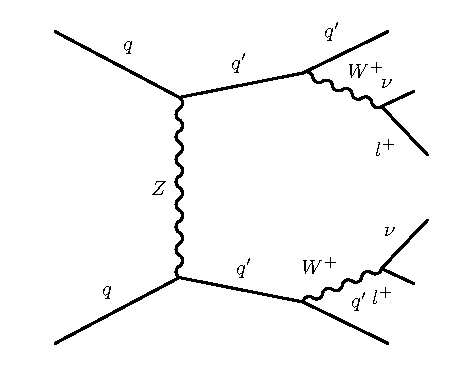
\includegraphics[width=0.35\textwidth]{figures/ss-exclboson-ww-diagram2.pdf}
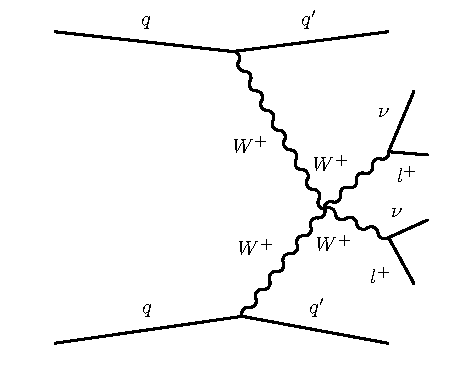
\includegraphics[width=0.315\textwidth]{figures/ss-exclboson-ww-diagram3.pdf}
\caption{
Representative Feynman diagrams for same-sign $WW$ production in association
with two jets from purely electroweak contributions:
(left) vector boson fusion,
(middle) bremsstrahlung-like,
and (right) multiperipheral production.
\label{fig:ss-exclboson-ww-sigdiagram}}

}
\end{figure*}


\begin{figure}[p]
    \centering
    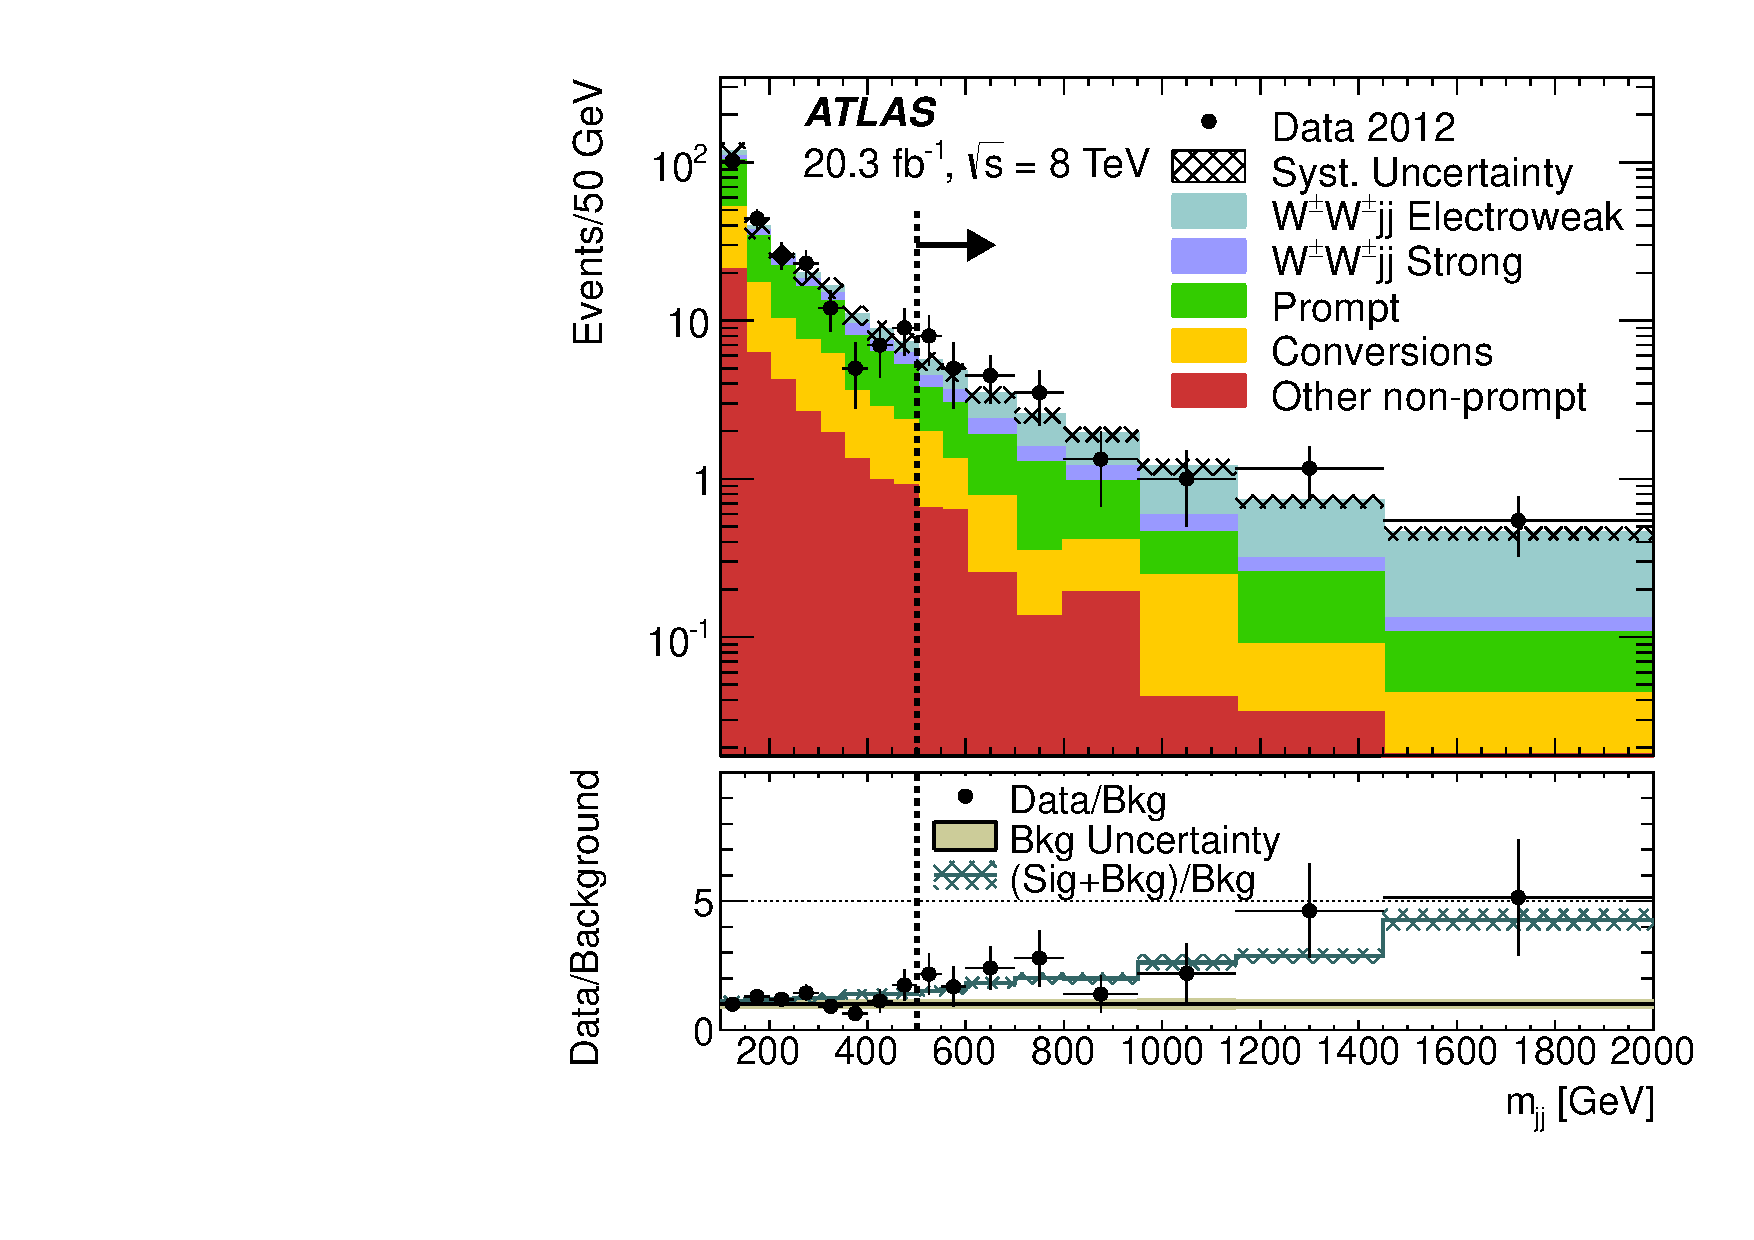
\includegraphics[width=0.45\textwidth]{figures/ss-exclboson-ww-ss-atlas8tev.pdf}
    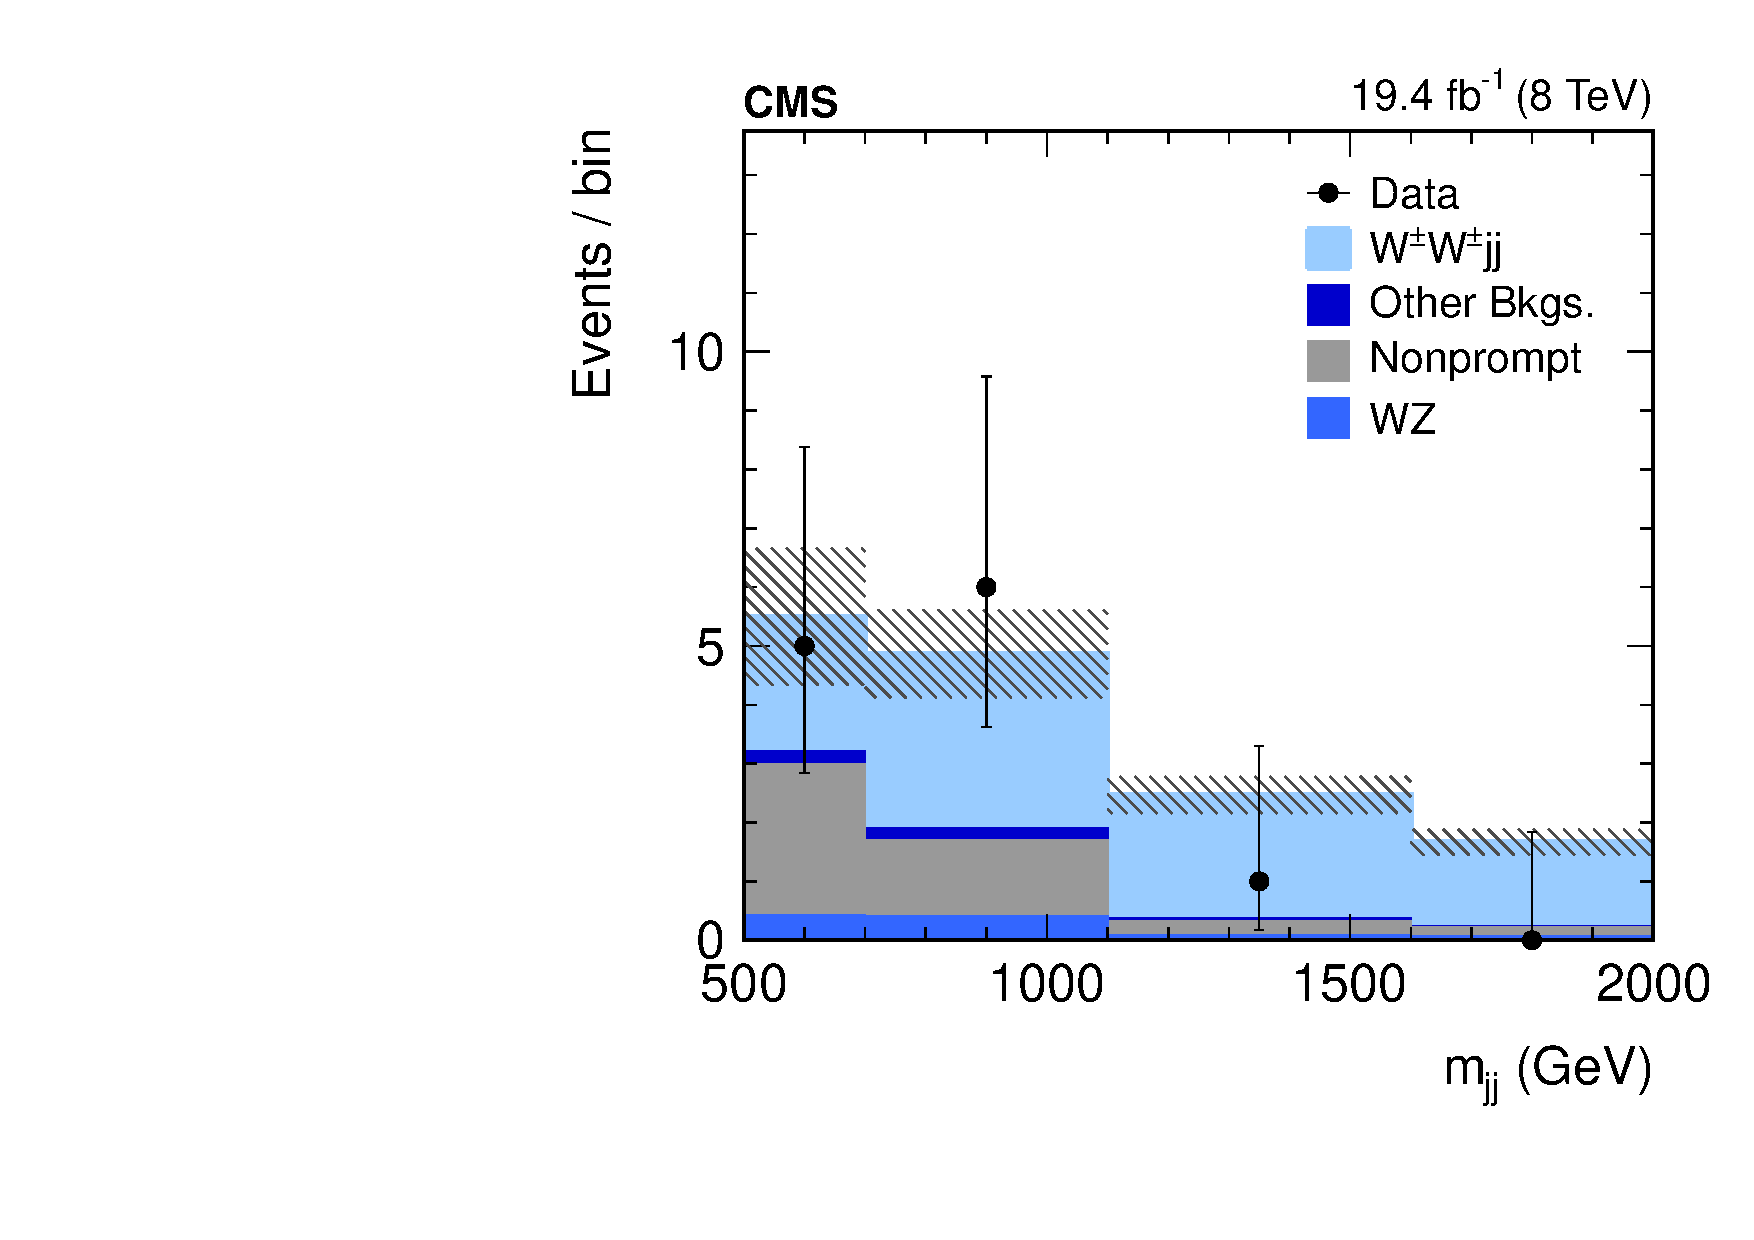
\includegraphics[width=0.45\textwidth]{figures/ss-exclboson-ww-ss-cms8tev.pdf}
    \caption{
    Left:  a signal region by ATLAS.
    Right:  }
    \label{fig:ss-exclboson-ww-ss}
\end{figure}
ATLAS SSWW 8 \TeV~\cite{Aad:2014zda}
CMS SSWW 8 \TeV~\cite{Khachatryan:2014sta}
